\chapter{GMAT's Estimation Subsystem}

\chapauthor{Stephen P. Hughes}{NASA/Goddard Space Flight Center}
\chapauthor{Darrel J. Conway}{Thinking Systems, Inc.}
\chapauthor{Matthew P. Wilkins}{Schafer Corporation}

In this chapter we present the highest level view of the proposed architectural design for
estimation functionality in GMAT.   We employ the Classes, Responsibilities, and Collaborations
(CRC) method discussed by Eckel\cite{thinkC} to describe the architecture.  We start by describing
the classes and their responsibilities.  For each class we present a brife description and a
bulleted list of primary responsibilities for instances of the class.  Then, we discuss the
allowable interactions and collaborations between the class instances.   A diagram is presented that
illustrates which classes/components can communicate with each other.  For each allowable
communication between classes, we discuss the reason for the interaction.

\section{Classes and their Responsibilities}

There are 10 classes designed or extended specifically for estimation that we discuss here.  These
classes are listed below.

\begin{itemize}
\item Resources
\begin{itemize}
\item Participants (Spacecraft, GroundStation, etc.)\footnote{The marked classes exist and are
extended to support estimation.}
\item Estimator
\item Measurement
\item Simulator
\item Propagator\footnotemark[\value{footnote}]
\item Event Locator
\end{itemize}
\item Commands
\begin{itemize}
\item RunEstimator
\item RunSimulator
\end{itemize}
\item Helpers
\begin{itemize}
\item Measurement Manager
\item State Manager
\item Propagation State Manager\footnotemark[\value{footnote}]
\item Estimation State Manager
\item File Reader and database*
\end{itemize}
\end{itemize}

Each class in this list has specific responsibilities and, with a few exceptions, all of the classes
above are employed to solve estimation problems in GMAT.  Next we will discuss the responsibilities
of each class.

\subsection{Resources}

\paragraph{Participants}  Participants are models of physical objects and processes that partake in
the measurement generation process.   For a GPS measurement, the participants are the user
spacecraft and the GPS constellation.  For an altimeter measurement the participants are the
spacecraft, and the central body.  Participants such as spacecraft and ground stations already exist
in GMAT, but will require modification to support estimation.  In the long term, participants such
as the TDRSS and GPS constellations and other Celestial bodies must be added to the system.

The classes for all measurement participants must contain specific functionality in order to support
the modeling of measurements and other estimation related models.    All participants must have
methods to get and set specific types of data such as state data, state transition matrix data, and
covariance data among others.  In summary, participants must support the following get/set methods:
\begin{itemize}
\item GetState() and SetState()
\item GetSTM() and SetSTM()
\item GetCovariance() and SetCovariance()
\end{itemize}

\paragraph{Estimator}  The estimator class is the base class for all estimators.  Estimators
take observed and computed measurement values, and potentially measurement partial derivatives, and
generate a sequence of state estimates until convergence or until stopping criteria are met.  The
estimator class contains the numerical methods such as batch least squares or the extended Kalman
filter.  In fact, most of the work involved in generating computed measurement values, including
evaluating measurement models, determining visibility conditions, and applying measurement
corrections, are invisible to the estimator class.  Those functions are performed by two helper
classes that provide bookkeeping and interfacing between the estimator and the measurement objects
and participants.  These helper classes are called the Estimator State Manager and the Measurement
Manager and are discussed below.  The primary responsibility of an Estimator is:
\begin{itemize}
\item Generate state estimates given observed and computed measurements, partial derivatives,
weights, and a-priori covariances.
\end{itemize}

\paragraph{Measurements}  The measurement class is the base class for all measurements.  For each
measurement type such as GPS, TDRSS, and ground station, there is a class derived from the
measurement base class.  Similarly, for each measurement data type such as GPS pseudorange, or
ground station right ascension and declination, there is a class derived from the appropriate parent
class such as GPSMeasurement or GroundStationMeasurement.  The measurement class performs modeling
of expected measurements, given the participants in the measurement process.  These modeling
functions include calculating expected measurement values including corrections, calculating
measurement partials, determining if the states of participants meet visibility and other conditions
that are required for measurement feasibility, and providing event function data for the iterative
determination of light time corrections.  In summary, the measurement classes have the following
responsibilities:
\begin{itemize}
\item Calculate expected measurement values and measurement partials given the participants
involved in the measurement process.
\item Determine if criteria are met for measurement feasibility.
\item Provide event function for tracking schedule generation and interface with event locator.
\item Provide event functions and interface with event locator for iterative determination of light
time correction, and propagation through deterministic event times such as averaging intervals.
\end{itemize}

\paragraph{Simulator}  The Measurement Simulator class simulates measurement observations.  To
perform its responsibilities, a simulator is provided a simulation time span and step size, a set of
desired measurements to simulate, and a list of participants for the measurements, along with a
propagator to use for propagation of the system.  Similar to the estimator class, most of the work
involved in generating simulated measurement values is invisible to the simulator class.  For
example, determining measurement feasibility, evaluating measurement models, and applying
measurement corrections and errors are performed by the measurement objects themselves.  To
summarize, the Estimator:
\begin{itemize}
\item Generate simulated measurement values.
\end{itemize}

\paragraph{Event Locater}  The event locater, implemented in the RootFinder class, is a helper class
for a propagator that controls propagation during the location of discrete events like eclipse
entry or exit, or measurement light time corrections.  In one mode, the event locater tracks event
function root values during propagation and lets the propagator know when a discrete event has been
bracketed.  To locate the event, iterative root finding methods on the event locater control the
propagation.  In summary, the responsibilities of the event locater are:
\begin{itemize}
\item Bracket event function roots by identifying two points that surround a root.
\item Iteratively solve for event function roots by controlling propagation steps.
\end{itemize}

\subsection{Commands}

\paragraph{RunSimulator}   GMAT includes components that are capable of generating simulated
data.  The Simulator, like all of GMAT's Solvers, implements a finite state machine.  The
Simulator's
state machine works with the RunSimulator command to calculate expected measurement values
and write these data to a measurement stream -- typically a simulated observation file.  In addition
to these tasks, the command performs the usual tasks assigned to members of GMAT's Mission
Control Sequence: checking for user actions such as hitting the stop or pause button, tracking the
execution location in the Mission Control Sequence, and managing object changes induced by
executing the command.  In summary, the responsibilities of the RunSimulator command are:
\begin{itemize}
\item Collaborate with an simulator to run the finite state machine defining the simulation process.
\item Perform initialization and finalization of the simulation processes.
\item Perform standard GMAT command actions.
\end{itemize}

\paragraph{RunEstimator}  The RunEstimator command is used to tell GMAT to solve an estimation
problem when events and maneuvers are not pat of the estimation process.  The user specifies an
estimator for the problem, and the RunEstimator command and the estimator work together to find an
estimate of state by executing the transitions in the estimator's finite state machine.  Depending
upon
the current finite state for the state machine (for example, the state machine may be in the
Initializing
state or the Calculating state, or one of several other states defined for that specific Estimator),
either
the RunEstimator Command or Estimator will be driving the estimation process. The RunEstimator
command also has basic housekeeping responsibilities required of all GMAT commands.  These
include checking for user actions such as hitting the stop button, tracking the execution location
in the
Mission Control Sequence, and managing object changes induced by executing the command.  In
summary, the responsibilities of the RunEstimator command are:
\begin{itemize}
\item Collaborate with an estimator to run the finite state machine defining the estimation process.
\item Perform initialization and finalization of the estimation processes.
\item Perform standard GMAT command actions
\end{itemize}

\subsection{Helper Classes}

\paragraph{MeasurementManager} The measurement manager (MM) is a helper class for the Estimator
and Simulator classes.  It performs data management and interfacing between the Solvers and the
measurement
objects.  A measurement manager has three areas of responsibility: sorting and bookkeeping observed
values that may come from numerous files or data streams, calling the appropriate measurement
object to determine computed measurement values and partial derivatives, and passing simulated data
to the measurement stream objects for storage and later use.  The Solvers do not
communicate directly with the measurement objects; instead, the MeasurementManager mediates that
communication.  The measurement manager coordinates measurement information flow among all the
measurement objects being used during an OD process.  The MM calls the file reader for each data
file and then sorts all observations into time-wise
order.  During the estimation process, the estimator calls the measurement manager and requests
observed and computed values at the current epoch, as well as the measurement partials.   The
measurement manager then calls the appropriate measurement to determine the computed
measurement value and the array of partial derivatives.  During simulation, it reverses this
process, calling the measurement objects to generate simulated observations, and then passing those
data to the file writers.  In summary, the measurement manager class
has the following responsibilities:
\begin{itemize}
\item Book keep observed values from observation data files and sort the observation data in time
order for use by the estimator.
\item Provide the estimator with a time ordered array of measurement epochs.
\item Provide the estimator with observed and computed measurement values, and partial derivatives
at the current measurement epoch.
\item Provide measurement weights to the estimator.
\item Receives generated measurement data and passes it to a data file writer or other output data
stream.
\end{itemize}

\paragraph{EstimatorStateManager}  The estimator state manager (ESM) retrieves state data from
objects involved in estimation and provides the data in a form ready for use by the estimator.
Hence, much of work performed by the ESM is getting and setting state data, including state
transition matrix and covariance information, so that the estimator methods do not have to interact
with all of the participant objects.  For example, after an iteration (for Batch) or state update
(for sequential), the ESM maps the new estimated state vector to the participating objects.
Similarly, when an estimator needs the STM, the ESM retrieves the portions of the STM from the
objects involved in estimation and assembles the complete STM and provides it to the Estimator.  In
summary, the responsibilities of the ESM class are:
\begin{itemize}
\item Get/Set state portions on objects involved in estimation and assemble the complete state
vector.
\item Get STM chunks from objects involved in estimation and assemble the total STM for the
estimator.
\item Get/Set state covariance chunks and assemble the entire covariance matrix.
\end{itemize}

\paragraph{File Reader/Writer}  The DataFile base class defines the methods and procedures to
provide data accessibility to other GMAT components. These methods include being able to move from
one data record to the next, as well as being able to request individual pieces of data without
knowledge of a specific data format.  The base class also provides general methods to appropriately
handle the basic categories of data formats.  The responsibilities of the file reader/writer class
are
\begin{itemize}
\item Read all or part of a date file.
\item Provide data of the requested type to the measurement object.
\item Write simulated data to the requested file format.
\end{itemize}

\paragraph{PropagatorStateManager}  The propagation state manager (PSM) retrieves state data from
objects involved in propagation and provides the data in a form ready for use by the propagator.
Hence, much of work performed by the PSM is getting and setting state data.  For example, after an
integration step the ESM maps the state vector to the participating objects.  Similarly, when a
propagator needs the initial state vector, the PSM retrieves the portions of the state from the
objects involved in propagation and assembles the complete state vector and provides it to the
propagator.  In summary, the responsibilities of the PSM class are:
\begin{itemize}
\item Get/Set state chunks on objects involved in propagation and assemble the complete state
vector.
\end{itemize}

\section{Collaboration between Classes}

The design of the estimation system limits interactions between components, in order to promote
loose coupling, a design principal used throughout GMAT.  Below, we discuss which components can
interact, and similarly, which components cannot interact.

There are three logical organizations of classes used in the orbit determination process:
\begin{itemize}
\item User configured resources
\item Estimation commands
\item Helper classes
\end{itemize}

Examples of resources include measurement participants (with attached sensors), measurements,
propagators, and estimators.  The helper classes include the EstimationStateManager (ESM),
Propagation State Manager (PSM), the Measurement Manager (MM), and the Event Locator (EL).
Currently, the only supported estimation commands are RunEstimator and RunSimulator.

Figure~\ref{fig:ODIneractions} contains an illustration all of the components involved in the
estimation process, and shows which components can interact via arrows between the components.   The
interactions are discussed in more detail below.

\begin{figure}[htbp]
\begin{center}
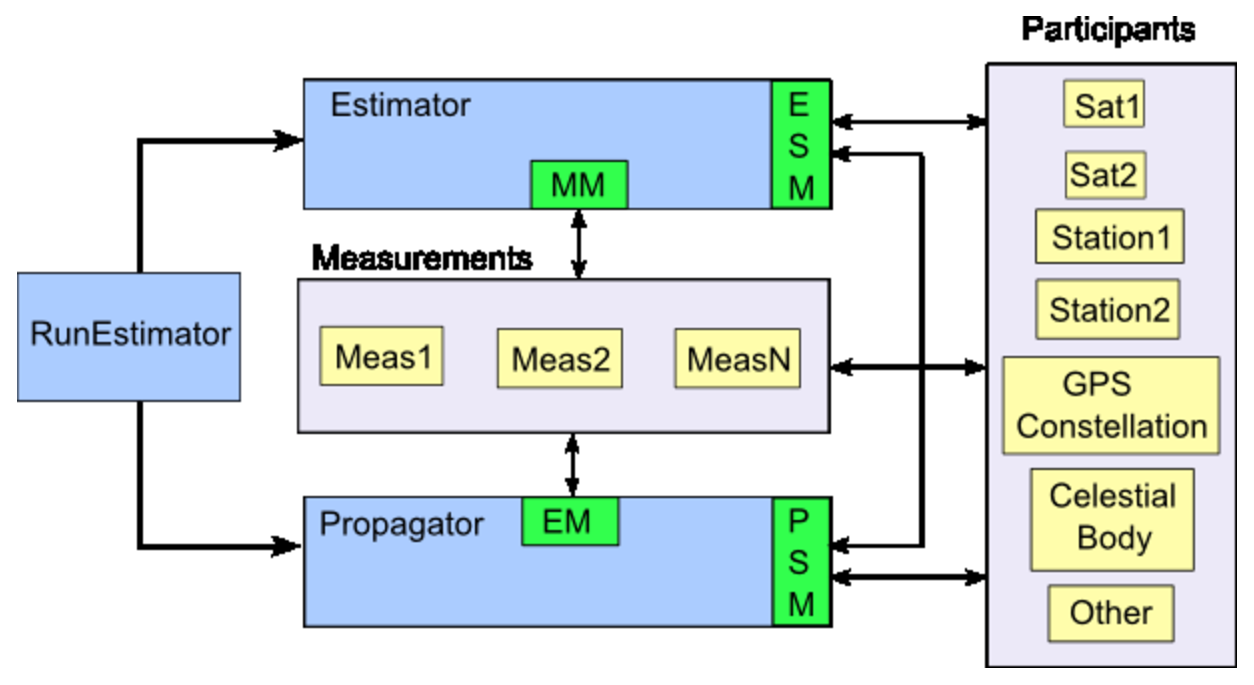
\includegraphics[scale=0.55]{Images/ODComponents.eps}
\caption{\label{fig:ODIneractions}OD Components and Interactions}
\end{center}
\end{figure}

\paragraph{Estimator -> ESM}  The ESM is an ``owned-object'' of an estimator.  The estimator
interacts with the ESM to get/set state related data from/on estimation participants.  The estimator
communicates with the ESM through several interfaces depending upon the type of state data such as
STM, covariance, or state vector.

\paragraph{ESM - >Participants}  The ESM communicates with participants to set and get state related
data.

\paragraph{Measurements->Participants}  Measurements communicate directly with measurement
participants/sensors.  Measurement objects have pointers to all measurement participants in the
measurement and therefore have direct access to public state data required to calculate measurement
values and partial derivatives.

\paragraph{PSM -> Participants}  The PSM communicates with participants to set and get state related
data.  This interface is similar to the ESM->Participants interface, except the PSM and ESM may not
manipulate the same state data.

\paragraph{ESM -> PSM}  The PSM and ESM interact during initialization.  The ESM provides the PSM
with a list of objects and IDs that are involved in the estimation process.  The PSM uses this
information to determine which states require propagation, and how those states should be propagated
(analytically or numerically).  In terms of the component level design, the PSM uses the data
provided by the ESM to generate the ListItem structure discussed in detail in the Component Design
section.

\paragraph{RunEstimator -> Propagator}  The RunEstimator command communicates with the propagator to
perform initialization and to propagate estimation participants.

\paragraph{RunEstimator -> Estimator}  The Estimator and the RunEstimator command function as a
finite state machine.  This is a complex interaction described in detail in later sections.

\paragraph{MM -> Measurements}  The measurement manager interacts with measurements during
initialization and execution.  During initialization, the measurement manager calls each measurement
object's Initialize() method and calls its GetObsData() method to get the arrays of epochs,
observations, and pointers to the measurement data objects.  During execution, the measurement
manager calls the Evaluate() and GetPartials() methods on the measurement object.

\paragraph{Estimator -> MeasurementManager}  The estimator interacts with the measurement manager to
get computed measurement values and partial derivatives and other measurement related information.

\section{Walkthrough of Sample Script Execution}

In this the remainder of this chapter, we present a simple estimation example in script form and
show at an intermediate level how GMAT would load and execute the script.  The first subsection
contains the sample script. The next subsection contains a general discussion of the steps GMAT uses
to execute any script.  We identify six key areas in the execution process that must be addressed in
the design of new estimation components and conclude the section with a more detailed discussion of
what happens for the new estimation components in those six key areas.  The design for the objects
used in this example are contained in the later chapters of this document.

\subsection{The Sample Script}

The sample script used for the execution walk-through has 5 objects:  a spacecraft named ODSat, a
ground station called Maui, a batch estimator called BLS, a measurement object named MauiData, a
propagator named ODprop, and a RunEstimator command.   The system processes range measurements
between Maui and ODsat using a batch least squares estimator.    The solve-for states are the
Cartesian states of the spacecraft.

\begin{quote}
\begin{verbatim}
%==========================================================================
%------  Define the spacecraft properties
%==========================================================================
Create Spacecraft ODSat;
ODSat.Id    = 21639;
ODSat.Epoch = 24228.72771990741;
ODSat.X     = 9882.164071524565;
ODSat.Y     = -23;
ODSat.Z     = 1837.579337039707;
ODSat.VX    = 0;
ODSat.VY    = 6.233189510799131;
ODSat.VZ    = 0.8480529946665489;
ODSat.OrbitCovariance = diag([100000^2*ones(3,1);1000^2*ones(3,1)]);

%==========================================================================
%==========================================================================
%------  Define the batch least squares solver
%==========================================================================
%==========================================================================
Create GroundStationMeasurement MauiData;
MauiData.Filename       = 'LEOMaui.mat';
MauiData.AddDataType = {'Range','ODSat','Maui'};

%==========================================================================
%------  Define the batch least squares solver
%==========================================================================
Create BatchEstimator BLS
BLS.MaxIterations   = 10;
BLS.RelTolerance    = 1e-5;
BLS.AbsTolerance    = 1e-5;
BLS.Measurements    = {'MauiData'};
BLS.SolveFor        = {'ODSat.CartesianState'};
BLS.Propagator      = 'ODProp';

%==========================================================================
%-----  Define the ground station properties
%==========================================================================
Create GroundStation Maui;
Maui.Id = 222;
Maui.X  = -4450.8;
Maui.Y  =  2676.1;
Maui.Z  = -3691.38 ;

%==========================================================================
%-----  Define the Propagator
%==========================================================================
Create ForceModel ODProp_ForceModel;
GMAT ODProp_ForceModel.CentralBody = Earth;
GMAT ODProp_ForceModel.PointMasses {Earth};

Create Propagator ODProp;
GMAT ODProp.FM = ODProp_ForceModel;
GMAT ODProp.Type = RungeKutta89;
GMAT ODProp.InitialStepSize = 60;
GMAT ODProp.Accuracy = 9.999999999999999e-12;

%==========================================================================
%-----  Solve the estimation problem
%==========================================================================
RunEstimator BLS;
\end{verbatim}
\end{quote}

\subsection{Overview of a GMAT Run}

\begin{figure}[htbp]
\begin{center}
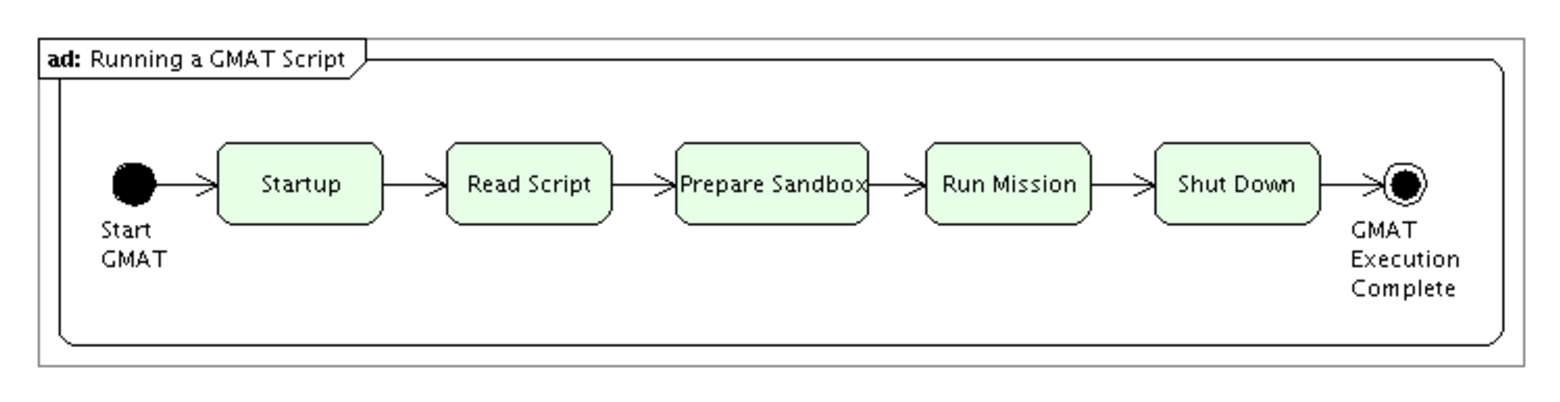
\includegraphics[scale=0.6]{Images/RunningaGMATScript.eps}
\caption{\label{fig:RunScript}GMAT Run Overview -- Running a Script}
\end{center}
\end{figure}

Figure~\ref{fig:RunScript} shows a high level view of the path through a run of a GMAT script.  When a user wants to run a GMAT script, she starts by opening the program, launching a set of actions that prepare the system for a run.  Once this startup process is complete, she loads the script into memory.  This script reading process creates the resources described in the script, loading them into GMAT's configuration (the container GMAT uses for objects created when building the resources in a script or from the GUI), and builds the commands in the Mission Control Sequence.  Next the objects are loaded into the Sandbox, and the Sandbox is prepared to perform the run by initializing all of the objects that were loaded.  The mission is run, executing the scripted sequence of commands. Finally, the user closes the program, completing the process.

\begin{figure}[htbp]
\begin{center}
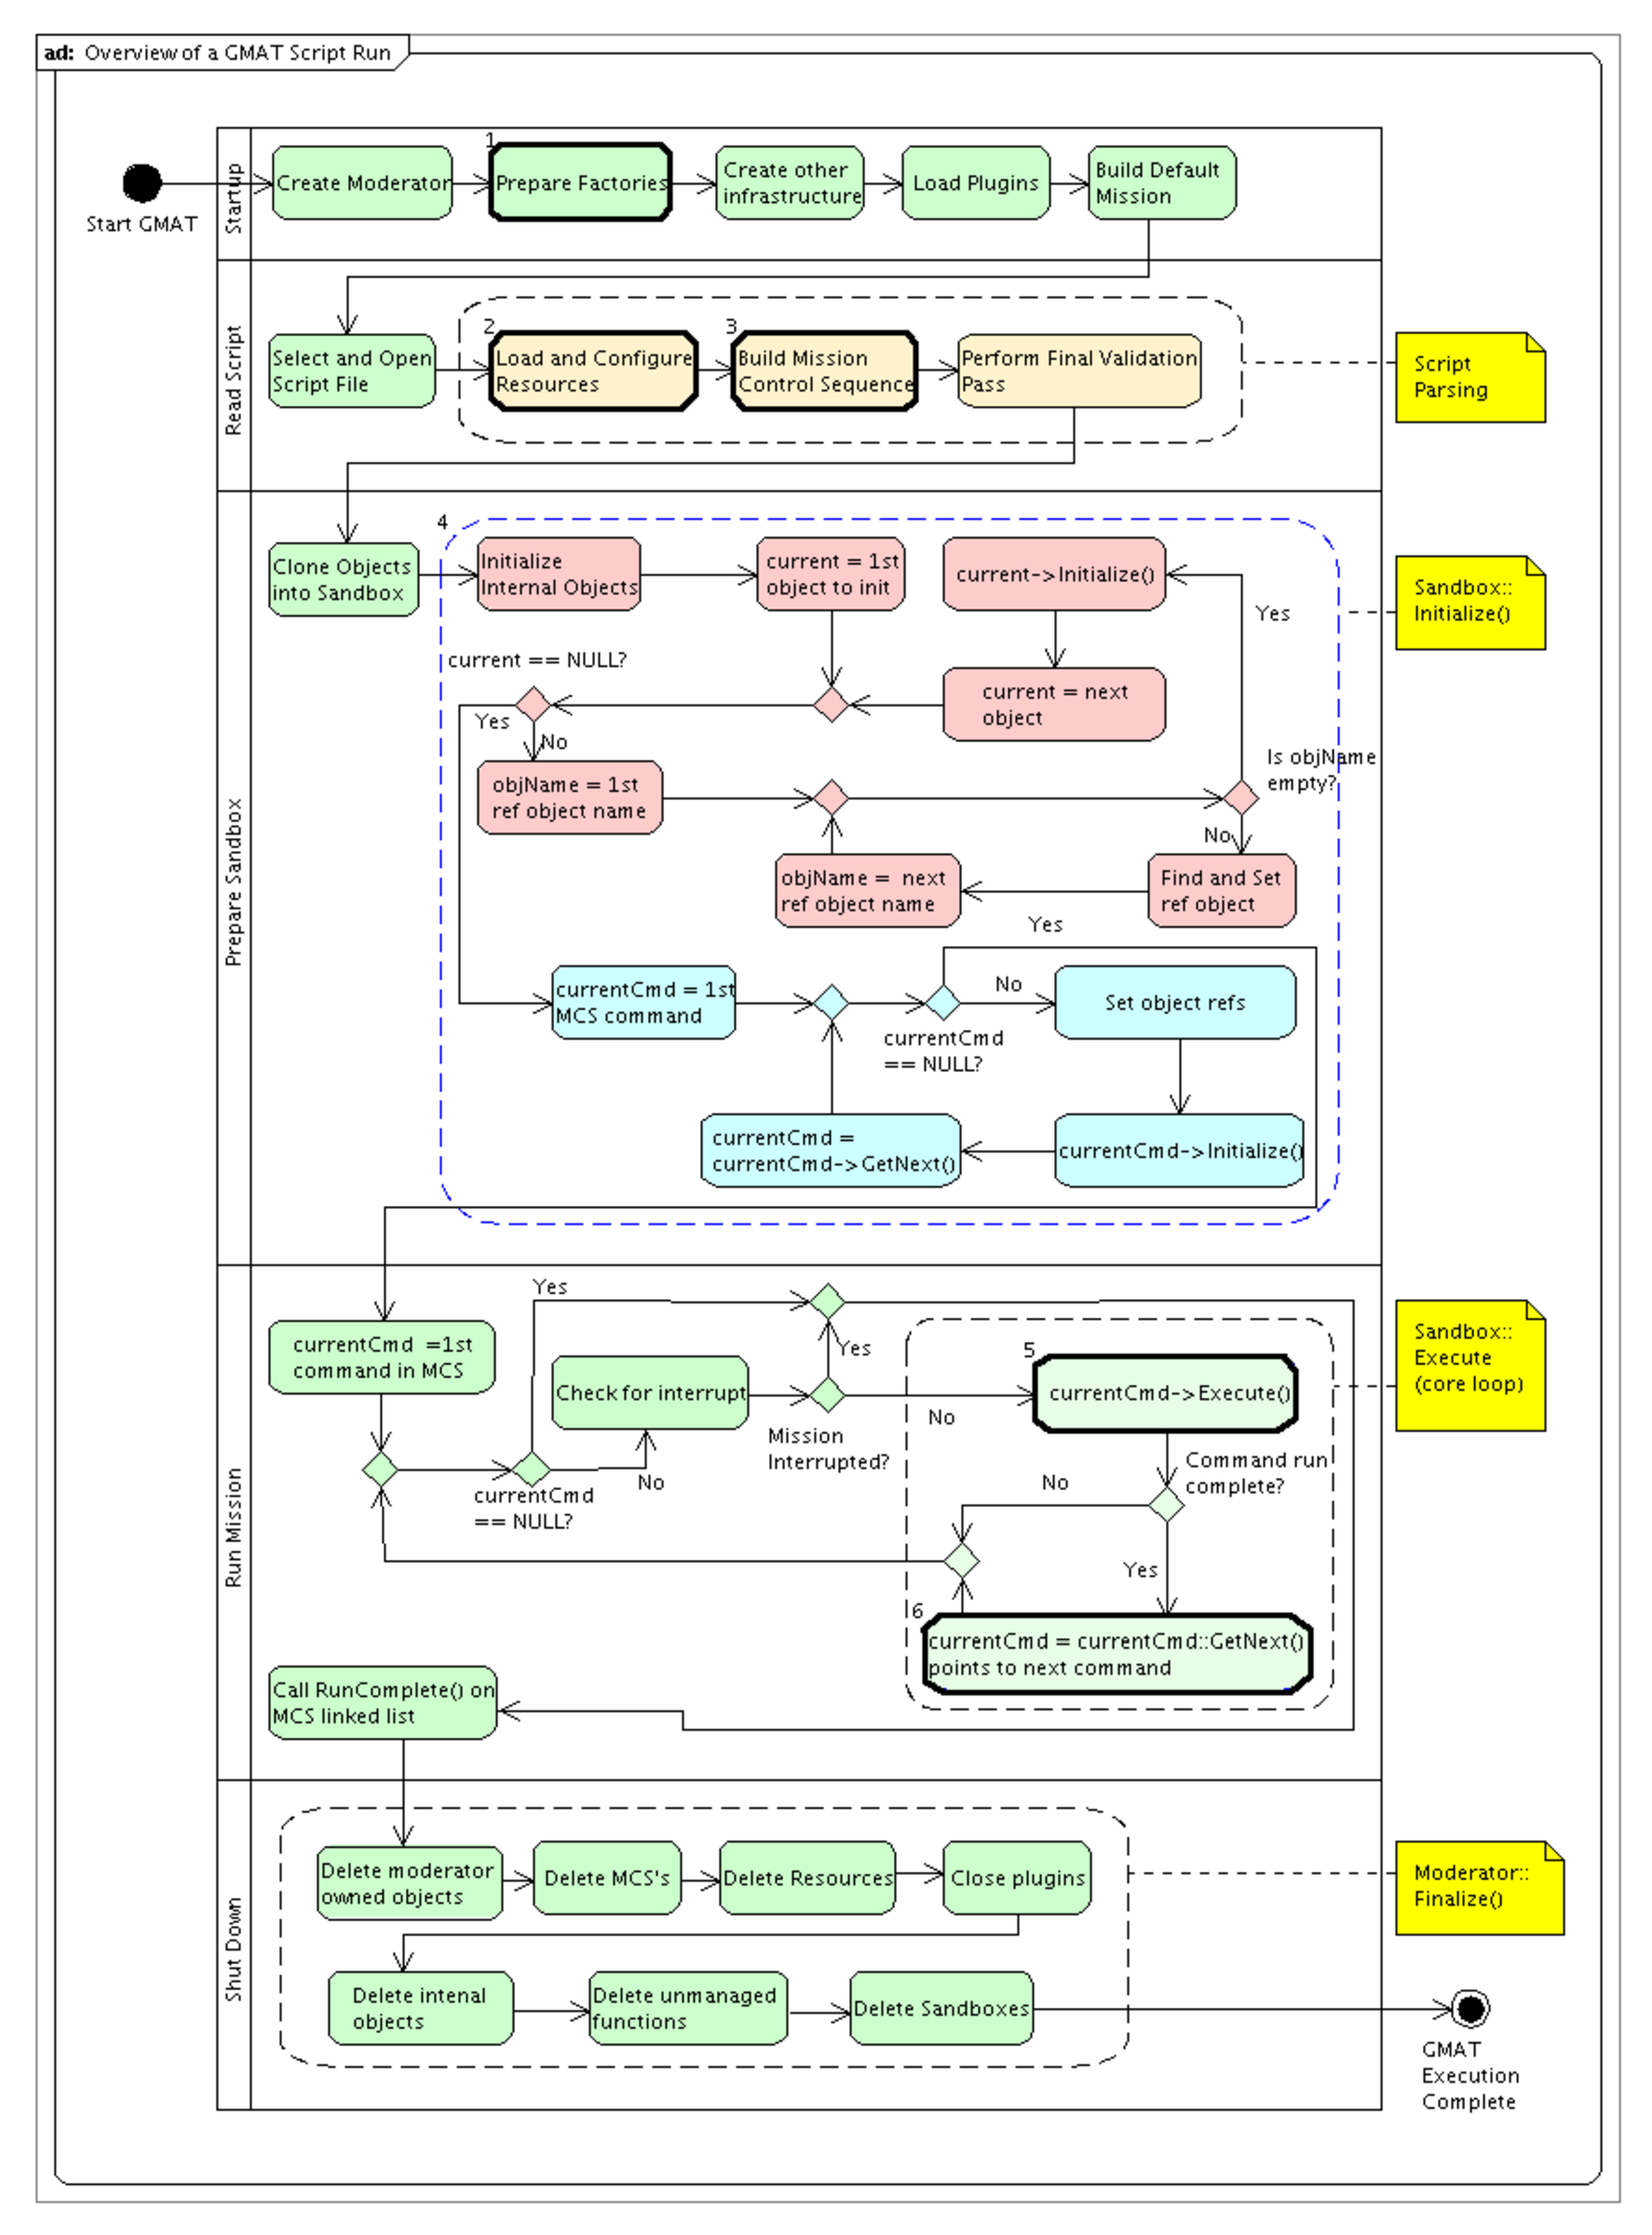
\includegraphics[scale=0.5]{Images/OverviewofaGMATScriptRun.eps}
\caption{\label{fig:RunScriptDetails}GMAT Run Overview -- Top Level Action Details}
\end{center}
\end{figure}

Figure~\ref{fig:RunScriptDetails} shows a first level expansion of these steps.  The details of the
steps shown in that figure can be found in the Architectural Specifications.  The blocks that are
affected by the new estimation components are numbered in the diagram, and will be discussed in more
detail in this document. There are six blocks that will be discussed here:

\begin{enumerate}
\item \textbf{Prepare Factories}  GMAT uses a set of components, called factories, to create
resources, commands for the Mission Control Sequence, and parameters used in calculations during a
mission run. New factories will be built to handle the new resources required to run estimation
problems in GMAT.
\item \textbf{Create and Configure Resources}  When GMAT parses a script, it reads the file one line
at a time, building the scripted objects and setting their parameters.  Depending on the resource,
the parameter setting phase may also include the creation and setting of objects owned by the
resource.
\item \textbf{Build Mission Control Sequence}  Following the resource definition and configuration
steps, the script describes the mission using a sequence of commands tailored to the components
supported by GMAT.  This sequence of commands is assembled into a linked list of objects called the
Mission Control Sequence.
\item \textbf{Prepare Sandbox}  GMAT runs missions inside of a component called the Sandbox.  When a
mission is run, the resources and Mission Control Sequence are loaded into the Sandbox used for the
run, interconnections between the components are established, and any pre-run data is set on these
components.  At the end of this process, the Sandbox is ready to execute the Mission Control
Sequence.
\item \textbf{Execute()}  Commands in the Mission Control Sequence manipulate the resources in the
Sandbox through a call to the Execute() method on each command in the sequence.
\item \textbf{GetNext()}  GMAT walks through the Mission Control Sequence by accessing the members
of the sequence's linked list.  Movement through the list is performed using the GetNext() method.
\end{enumerate}

These above six portions of a GMAT run are particularly relevant to the new estimation components.
The remaining blocks in the diagram may be discussed in passing, but the focus of the descriptions
necessary to build the pieces GMAT needs will include discussion of these six elements in more
detail.

The sample script presented earlier contains five resources and a command: a Spacecraft named ODSat,
a Measurement named MauiData (which contains two owned data members, a MeasurementReader and a
GroundstationRange MeasurementData object), a BatchEstimator named BLS, a GroundStation named Maui,
a Propagator named ODProp (with an owned ForceModel), and a RunEstimator command.  The estimator
contains a MeasurementManager and an EstimationStateManager as member objects.  Similarly, the
propagator contains instances of a PropagationStateManager and an EventLocator.  Each of the
following sections will conclude with a table reporting the status of GMAT and each of these six
objects after the process described in the section has acted on the sample script.  Prior to launch
of the system, the system description table looks like this:
\begin{center}
\begin{tabular}{|p{1in}|p{1.5in}|p{3in}|}
\hline\mc{3}{|l|}{\cellcolor[rgb]{0.75,0.75,0.75}\textbf{GMAT Status Before Starting the
Program}} \\
\hline\mc{3}{|p{5.5in}|}{The program has not yet started} \\
\hline\rowcolor[rgb]{0.9,0.9,0.9}\textbf{\textit{Object}} & \textbf{\textit{Status}} &
\textbf{\textit{Notes}} \\
\hline ODSat & Not yet created &  \\
\hline MauiData & Not yet created &  \\
\hline BLS & Not yet created & Once built, includes an EstimationStateManager and a
MeasurementManager as members \\
\hline Maui & Not yet created &  \\
\hline ODProp & Not yet created & Once built, includes a PropagationStateManager and an EventLocator
as members \\
\hline RunEstimator & Not yet created & \\
\hline
\end{tabular}
\end{center}

\subsection{Script Execution Walkthrough}

\subsubsection{Block 1: Prepare Factories}

GMAT's Factory subsystem is used to create all scriptable components of the system.  The subsystem
is an implementation of the Abstract Factory design pattern: it defines the interfaces used for
creating user objects and Mission Control Sequence commands, and uses derived Factory classes to
provide the implementation for specific class instantiations.  The Factory subsystem is managed by a
singleton instance of the FactoryManager class.  The Moderator calls methods on the FactoryManager
to create instances of specific types of objects, identified by the name of the object's type:
Spacecraft, GroundStation, DifferentialCorrector, and so forth.  Similarly, the Moderator calls the
FactoryManager to create instances of GMAT's command classes in order to build the Mission Control
Sequence.

Each Factory supporting user objects is registered with the FactoryManager when GMAT starts up.  The
internal factories are registered first, followed by factories contained in plug-in libraries.  The
addition of estimation capabilities to GMAT necessitates the construction of factories supporting
the new types of objects that are used for estimation, along with registration of these new
factories with the FactoryManager.  The ``Prepare Factories'' block of the master overview diagram
(Figure~\ref{fig:RunScriptDetails}) identifies the location of the factory registration in the life
cycle of a GMAT run.

Estimation requires the construction of five (check this) new factories for the internal
capabilities being designed here.  These new factories are:
\begin{itemize}
\item \textbf{EstimatorFactory}  The Factory that creates GMAT's internal estimators.  These
components could be added directly to the SolverFactory, since all Estimators are Solvers.  The
inclusion of a new factory for the Estimator objects keeps the factory subsystem more modular, and
will allow for inclusion of the estimation capabilities as a plug-in if desired.
\item \textbf{MeasurementFactory}  Measurement objects, a new class of object in GMAT, require a new
Factory supporting their instantiation.  The Measurement objects include elements that define data
types for the measurements and sources for observation data.  Separate factories are provided for
these elements.
\item \textbf{MeasurementDataFactory}  Creates the measurement data objects.  The measurement data
objects are used to calculate the expected value of a specific type of measurement along with the
partial derivatives associated with that value.
\item \textbf{ObservationReaderFactory}  Creates the objects used to read and write observation
data.  The observation data may be fed into GMAT from a data file, a database, or by means of a live
data feed.  The initial builds of GMAT's estimation subsystem are designed to work using data from a
file.
\item \textbf{EstimationCommandFactory}  Creates the commands used in estimation. The inclusion of a
new factory for the estimation commands objects keeps the factory subsystem more modular, and will
allow for inclusion of the estimation capabilities as a plug-in if desired.
\end{itemize}

The Moderator creates these factories during system start\footnote{Internal and plug-in factories
are constructed and registered in the Moderator's initialization code.  The Estimation
 code is built as a plug-in module, and as such, is loaded into the system by loading the library
at run time after all of the internal Factory objects have been loaded.}.  Each factory is passed
to the FactoryManager once it is created. The FactoryManager obtains the base type of the objects
supported by the factory along with a list of the supported types.  For example, in the initial
estimation release, the MeasurementDataFactory will report that it supports the
Gmat::MEASUREMENT\_DATA type, and can supply specific objects for ``GroundStationRange'',
``GroundStationRangeRate'', ``GroundStationRADec'', and ``GroundStationAzEl'' measurement data.

The factories identified above will be described in more detail in the class descriptions.  These
factories follow the same pattern as is found in the rest of GMAT.  There are no special
considerations imposed on the system by the inclusion of the estimation related factories.

Several new base object types will be added to GMAT to support estimation.  Specifically, new types
will be added to support Measurement classes, MeasurementData classes, and ObservationReader
classes.  (The Estimator classes are already handled through inheritance from the Solver base
class.)  The Factory base class and Gmat namespace will be extended to include these new types.

The following table shows the configuration of GMAT and the state of each of the objects contained
in the sample script after the factory registration phase is complete.

\begin{center}
\begin{tabular}{|p{1in}|p{1.5in}|p{3in}|}
\hline\mc{3}{|l|}{\cellcolor[rgb]{0.75,0.75,0.75}\textbf{GMAT Status After Preparing Factories}} \\
\hline\mc{3}{|p{5.5in}|}{This step prepares the elements of GMAT's engine that are needed to build
the resources and commands in a GMAT script.  All of the factories have been created and registered
with GMAT's FactoryManager.  GMAT is essentially idle, waiting for a user prompt to begin
processing.  The GUI versions of GMAT complete the system startup by building the default mission.}
\\
\hline\rowcolor[rgb]{0.9,0.9,0.9}\textbf{\textit{Object}} & \textbf{\textit{Status}} &
\textbf{\textit{Notes}} \\
\hline ODSat & Not yet created &  \\
\hline MauiData & Not yet created &  \\
\hline BLS & Not yet created & \\
\hline Maui & Not yet created &  \\
\hline ODProp & Not yet created & \\
\hline RunEstimator & Not yet created & \\
\hline
\end{tabular}
\end{center}

\subsubsection{Block 2: Load and Configure Resources}

The objects users configure in GMAT fall into two categories: Resources and Commands.  The elements
that define the time ordered sequence of actions in the Mission Control Sequence fall into the
latter category, and are discussed in the Block 3 description below.  The elements that identify the
physical objects and tools that manipulate those objects are called resources.  These components
include the Spacecraft; Groundstations; hardware elements (tanks and thrusters); celestial bodies
and special locations in the solar system; variables, arrays, and strings; targeters, optimizers,
and estimators; and other elements that act as items used when defining the mission timeline.  In
the GUI versions of GMAT, these pieces are located on the Resources tree, while the commands appear
on the Mission tree.

GMAT's script processing subsystem operates in two distinct modes: object mode and command mode.
The resources are created and configured in object mode, prior to the definition of the Mission
Control Sequence.  As soon as a command for the Mission Control Sequence is encountered, the
ScriptInterpreter changes from object mode into command mode.  Each subsequent line of the script
file is treated as a node in the control sequence, and placed into the linked list defining the
Mission Control Sequence.

Block 2 in the master overview diagram represents the actions taken by the ScriptInterpreter in
object mode.  In this mode, GMAT creates resources, saves them for later use, and sets parameters on
created resources.  Resources are built from script lines that start with the GMAT keyword
``Create''. When the ScriptInterpreter finds a line starting with that keyword, it takes the next
word in the line as the text describing the type of object requested, and the remaining words as the
names of objects of the specified type that need to be constructed.  The ScriptInterpreter passes
the request for each new object to the Moderator, which passes the request into GMAT's
FactoryManager.  The FactoryManager locates the factory responsible for creating the requested
object type, and passes the creation request into that factory.  The factory creates the requested
object, assigning it the specified name, and returns the new object's pointer to the Moderator.  (If
no object was created, the returned pointer is NULL.)  The Moderator passes the object into the
ConfigurationManager so that the new object can be stored for later use (objects managed this way by
the ConfigurationManager are referred to as ``configured objects''), and then returns the pointer to
the ScriptInterpreter.

Assignment lines -- that is, lines of the form ``object.parameter = value'' -- encountered in object
mode make calls directly into the configured objects, setting values on those objects.  This
parameter setting identifies values used by the objects, sets the identities for references the
objects use, and in some instances sets up owned objects that the configured objects need.  If an
object uses a reference to another configured object, the name of the referenced object is stored as
a string in the object that uses the reference so that the object pointer can be set during
initialization in GMAT's Sandbox.  For example, when the script line ``BLS.Propagator = ODProp;'' is
parsed, the BLS estimator is sent the string 'ODProp'.  The BLS propagator stores that string name
for use during the ``Prepare Sandbox'' phase to identify the propagator object that the estimator
needs.

Most of the object parameter setting needed by the estimation resources fall into the category of
parameter values and references set by object name.  Discussions for this type of parsing will not
be presented in detail in this document for all of the estimation components.  The components that
use owned objects will contain information detailing the creation and configuration of those
objects.  In particular, the Measurement objects own MeasurementData objects and ObservationReader
objects in order to provide calculated and observed data and derivative information to the
estimation process.  The management of these elements will be discussed in the class descriptions
below.

\begin{center}
\begin{tabular}{|p{1in}|p{1.5in}|p{3in}|}
\hline\mc{3}{|l|}{\cellcolor[rgb]{0.75,0.75,0.75}\textbf{GMAT Status After Creating and Configuring
Resources}} \\
\hline\mc{3}{|p{5.5in}|}{The resources defined in the script have been created, and all of the
object properties defined for these resources have been set.  Internal (``owned'') objects defined
for the resources have been created and set on the resources.  The next script line that is read
describes the first command in the Mission Control Sequence.  It will toggle the ScriptInterpreter
out of object mode and into command mode.} \\
\hline\rowcolor[rgb]{0.9,0.9,0.9}\textbf{\textit{Object}} & \textbf{\textit{Status}} &
\textbf{\textit{Notes}} \\
\hline ODSat & Created, Properties Set, Uninitialized & Scripted data values have been set. \\
\hline MauiData & Created, Properties Set, Uninitialized & The owned ObservationReader and
GroundstationRange objects have also been created and passed to MauiData.  The file handle for the
ObservationReader has not yet been opened.  \\
\hline BLS & Created, Properties Set, Uninitialized & Scripted data values have been set.  The names
of reference objects are set.  The pointers to the reference objects are all NULL.  The BLS
MeasurementManager and EstimationStateManager are created as part of the estimator, but not
initialized.  The EstimationStateManager and MeasurementManager objects have been created as object
members.  Neither contains any data. \\
\hline Maui & Created, Properties Set, Uninitialized & Scripted data values have been set. \\
\hline ODProp & Created, Properties Set, Uninitialized & Scripted data values have been set.  The
ODProp PropagationStateManager and EventLocator have been created as part of the propagator, but not
yet initialized. \\
\hline RunEstimator & Not yet created & \\
\hline
\end{tabular}
\end{center}

\subsubsection{Block 3:  Build Mission Control Sequence}

Resources in GMAT are built by the ScriptInterpreter running in object mode.  As soon as GMAT finds
a Mission Control Sequence command in the script file, it toggles into command mode, and remains in
that mode until the script has been fully read.  Commands in GMAT can be interpreted in one of two
different ways.  Commands that are scripted using a simple series of strings with no specialized
elements follow this format:
\begin{quote}
commandKeyword [element1 ...]
\end{quote}

(The formatting here is that optional elements lie in square brackets, and ellipses indicate
additional pieces matching the one preceding the ellipses.  If a selection is necessary between
several options, the choices are separated by a vertical bar.)  Commands formatted this way can be
handled directly by the ScriptInterpreter.  Commands that have more specialized syntax override the
GmatCommand::InterpretAction() method and provide customized parsing for the line of text defining
the command.

The estimation commands planned for the initial releases of GMAT's new capabilities, RunEstimator
and RunSimulator, fall into the former category.  These commands are passed a single command
parameter and possibly a mode string defining the mode of operation.  Details about the syntax for
each of these commands can be found in the descriptions of the command classes, later in this
document.

\begin{center}
\begin{tabular}{|p{1in}|p{1.5in}|p{3in}|}
\hline\mc{3}{|l|}{\cellcolor[rgb]{0.75,0.75,0.75}\textbf{GMAT Status After Building the Mission
Control Sequence}} \\
\hline\mc{3}{|p{5.5in}|}{This step completes the script reading phase of the Interpreter's work.
All that remains is the final pass through the objects to validate a few settings and to ensure that
all of the objects needed to run actually do exist in the ConfigurationManager's object container.}
\\
\hline\rowcolor[rgb]{0.9,0.9,0.9}\textbf{\textit{Object}} & \textbf{\textit{Status}} &
\textbf{\textit{Notes}} \\
\hline ODSat & Created, Properties Set, Uninitialized &  \\
\hline MauiData & Created, Properties Set, Uninitialized &  \\
\hline BLS & Created, Properties Set, Uninitialized &  \\
\hline Maui & Created, Properties Set, Uninitialized &  \\
\hline ODProp & Created, Properties Set, Uninitialized &  \\
\hline RunEstimator & Created, Properties Set, Uninitialized & The referenced Estimator, ODProp, is
identified by name.  The pointer is not set. \\
\hline
\end{tabular}
\end{center}

\subsubsection{Block 4:  Prepare Sandbox}

GMAT runs scripts in an instance of a specialized container class called the Sandbox.  The process
of running a script is performed in two phases: Sandbox Initialization and Sandbox Execution.  The
initialization phase consists of four steps, shown in Figure~\ref{fig:SandboxInitialization}.

\begin{figure}[htbp]
\begin{center}
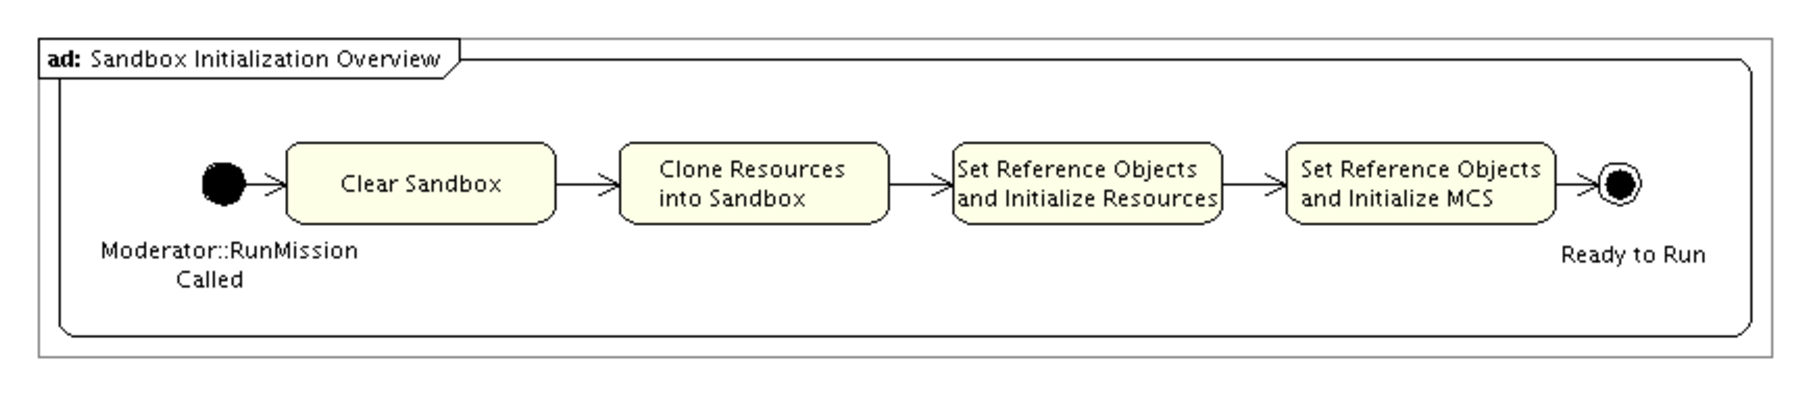
\includegraphics[scale=0.5]{Images/SandboxInitializationOverview.eps}
\caption{\label{fig:SandboxInitialization}Steps in the Sandbox Initialization Process}
\end{center}
\end{figure}

First, the Sandbox is instructed to clear its data structures in case there are objects in the Sandbox from a previous script execution.  Next, all of the resources managed by the
ConfigurationManager are copied into the Sandbox.  The original configured objects are not moved into the Sandbox; instead, the Sandbox makes a copy of each object for local use in the Sandbox, using each resource's Clone() method.  The Mission Control Sequence is also passed into the Sandbox at this time; the Mission Control Sequence is not cloned.

Once all of the resources have been cloned into the Sandbox, the Sandbox's Initialize() method is called.  This method initializes the resources and commands for use in the mission run.  The Sandbox performs this initialization of resources in an ordered fashion, ensuring that more basic resources are initialized before the components that use them are initialized\footnote{Resource initialization is actually handled in an instance of the ObjectInitializer class in the Sandbox.  The ObjectInitializer manages the ordered initialization process, which is performed as described here.}.  The resource initialization is performed one object at a time.  Resource initialization consists of three steps: (1) the Sandbox retrieves a list of objects referenced by the object that is being initialized, (2) each object in the list of references is located and passed by pointer to the object being initialized, and (3) the object's Initialize() method is called.

Steps (1) and (2) described here are illustrated in the system specifications\cite{archSpec}.  The Sandbox contains two object containers: the objectMap containing objects specific to the Mission Control Sequence but not automatically visible to functions in the control sequence, and the globalObjectMap containing objects visible to all commands in the Sandbox, including those in function calls.  This object scoping complexity is managed as part of the Sandbox initialization process.

\begin{figure}[htbp]
\begin{center}
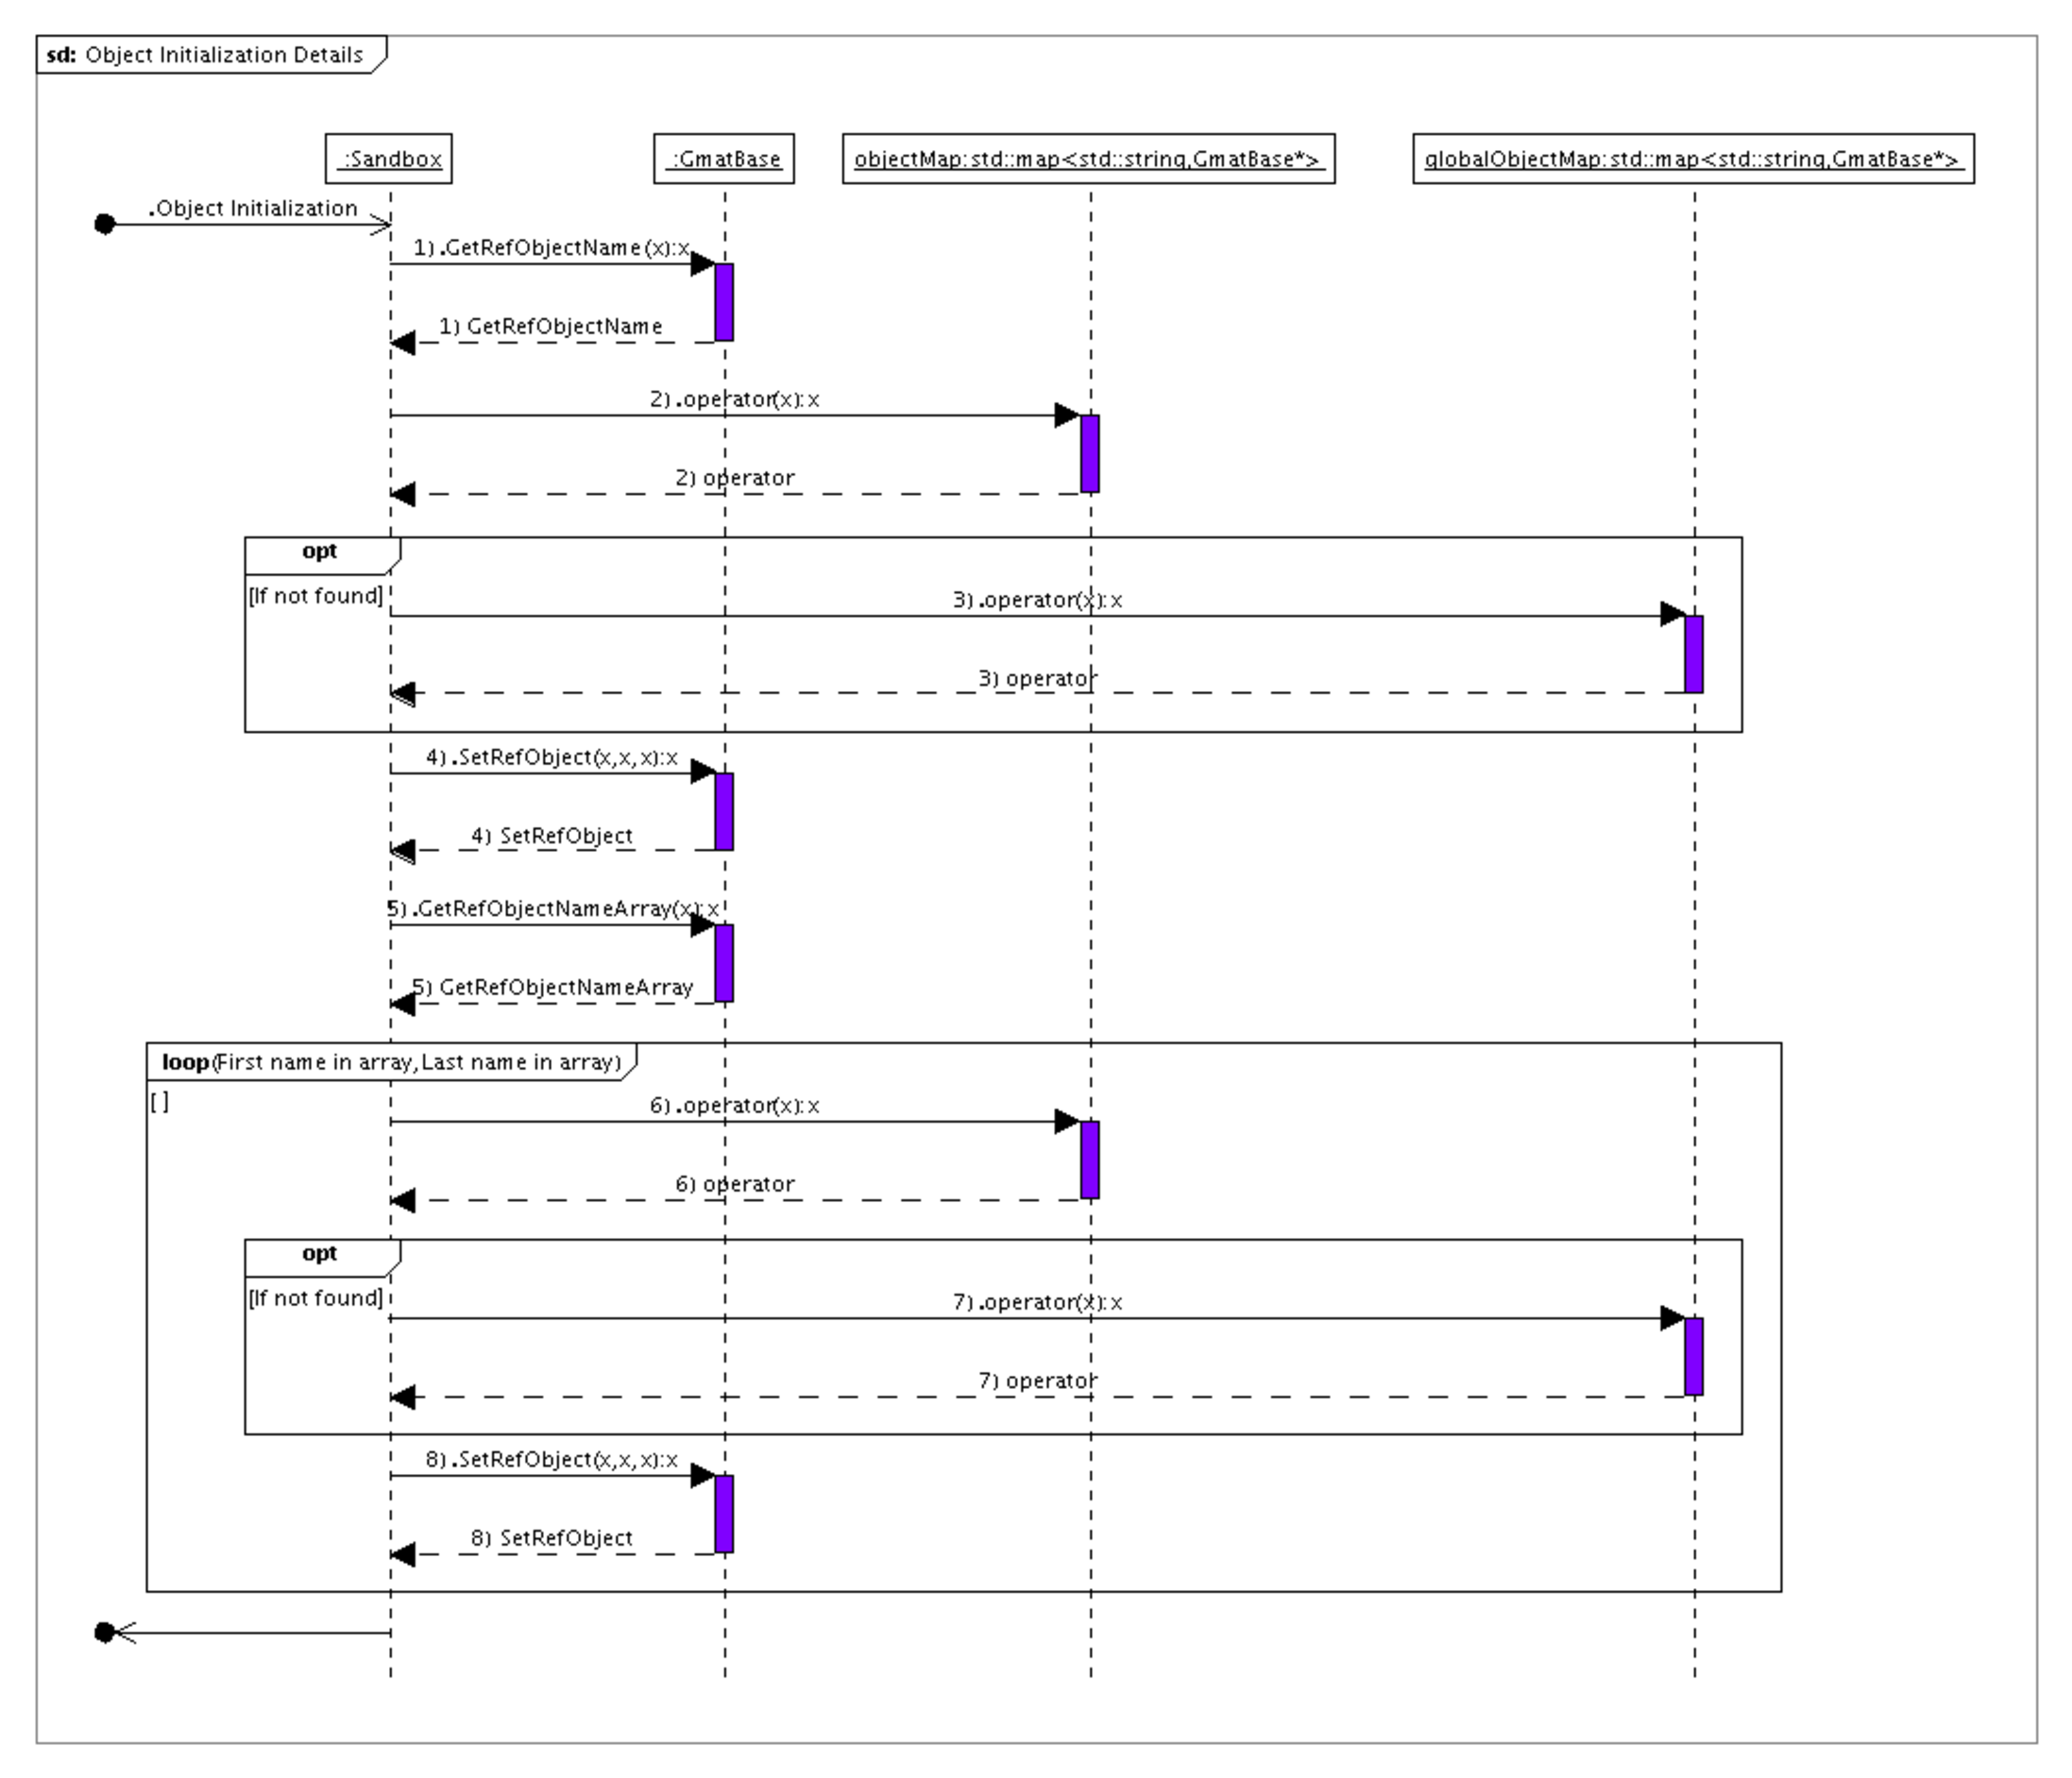
\includegraphics[scale=0.45]{Images/ObjectInitializationDetails.eps}
\caption{\label{fig:ObjectInitializationDetails}Reference Object Setting during Initialization}
\end{center}
\end{figure}

Objects in GMAT may contain object references that are accessed in one of two ways.  Objects with a single referenced object provide the Sandbox with the name of that object through a call to the GetRefObjectName() method.  Objects that reference multiple references provide a StringArray of reference objects names through a call to the GetRefObjectNameArray() method.  The calls made in the Sandbox to access these two methods are also shown in Figure~\ref{fig:ObjectInitializationDetails}.

After all of the resources have been initialized, the Sandbox initializes the Mission Control Sequence.  Control sequence initialization is performed one command at a time, using a pointer to the current command being initialized.  This process is performed in three steps.  First, the current command is passed a pointer to the solar system used in the Sandbox, the internal object pointers, and the arrays of the resources that were cloned into the Sandbox.  Once the command has these pointers set, it initializes itself through a call to its Initialize() method.  Finally, the current command pointer is updated to point to the next command that needs initialization through a call to the GetNext() method.

Sandbox initialization is the most complicated phase of a mission run in GMAT.  Because of this complexity, the initialization steps required for each of the new estimation objects will be described in the class descriptions below.

\begin{center}
\begin{tabular}{|p{1in}|p{1.5in}|p{3in}|}
\hline\mc{3}{|l|}{\cellcolor[rgb]{0.75,0.75,0.75}\textbf{GMAT Status After Preparing the Sandbox for the Run}} \\
\hline\mc{3}{|p{5.5in}|}{ Mission runtime copies of all resources and commands have been passed into the Sandbox.  Each resource has had its references to other resources set.  The Mission Control Sequence has been passed the local and global object stores (named objectMap and globalObjectMap in the code), and used these structures to locate and set pointers to the objects used by each command in the sequence.  GMAT is ready to run the mission. } \\
\hline\rowcolor[rgb]{0.9,0.9,0.9}\textbf{\textit{Object}} & \textbf{\textit{Status}} &
\textbf{\textit{Notes}} \\
\hline ODSat & Created and Initialized & All resources here are clones of the configuration
manager's objects.  Pointers to the referenced objects have all been set. \\
\hline MauiData & Created and Initialized &  \\
\hline BLS & Created and Initialized &  \\
\hline Maui & Created and Initialized &  \\
\hline ODProp & Created and Initialized &  \\
\hline RunEstimator & Created and Initialized & The pointer to the estimator has now been set. \\
\hline
\end{tabular}
\end{center}

\subsubsection{Block 5:  Execute() and Block 6:GetNext()}

Upon completion of the Prepare Sandbox step described above, all of the pointers connecting the objects together for the mission run have been set, and each element of the run has been given the opportunity to perform its initialization.  The commands in the Mission Control Sequence have all been passed pointers to the objects used to run the mission, and have been given the opportunity to perform their initialization.  The Mission Control Sequence is ready to run the mission.

\begin{figure}[htbp]
\begin{center}
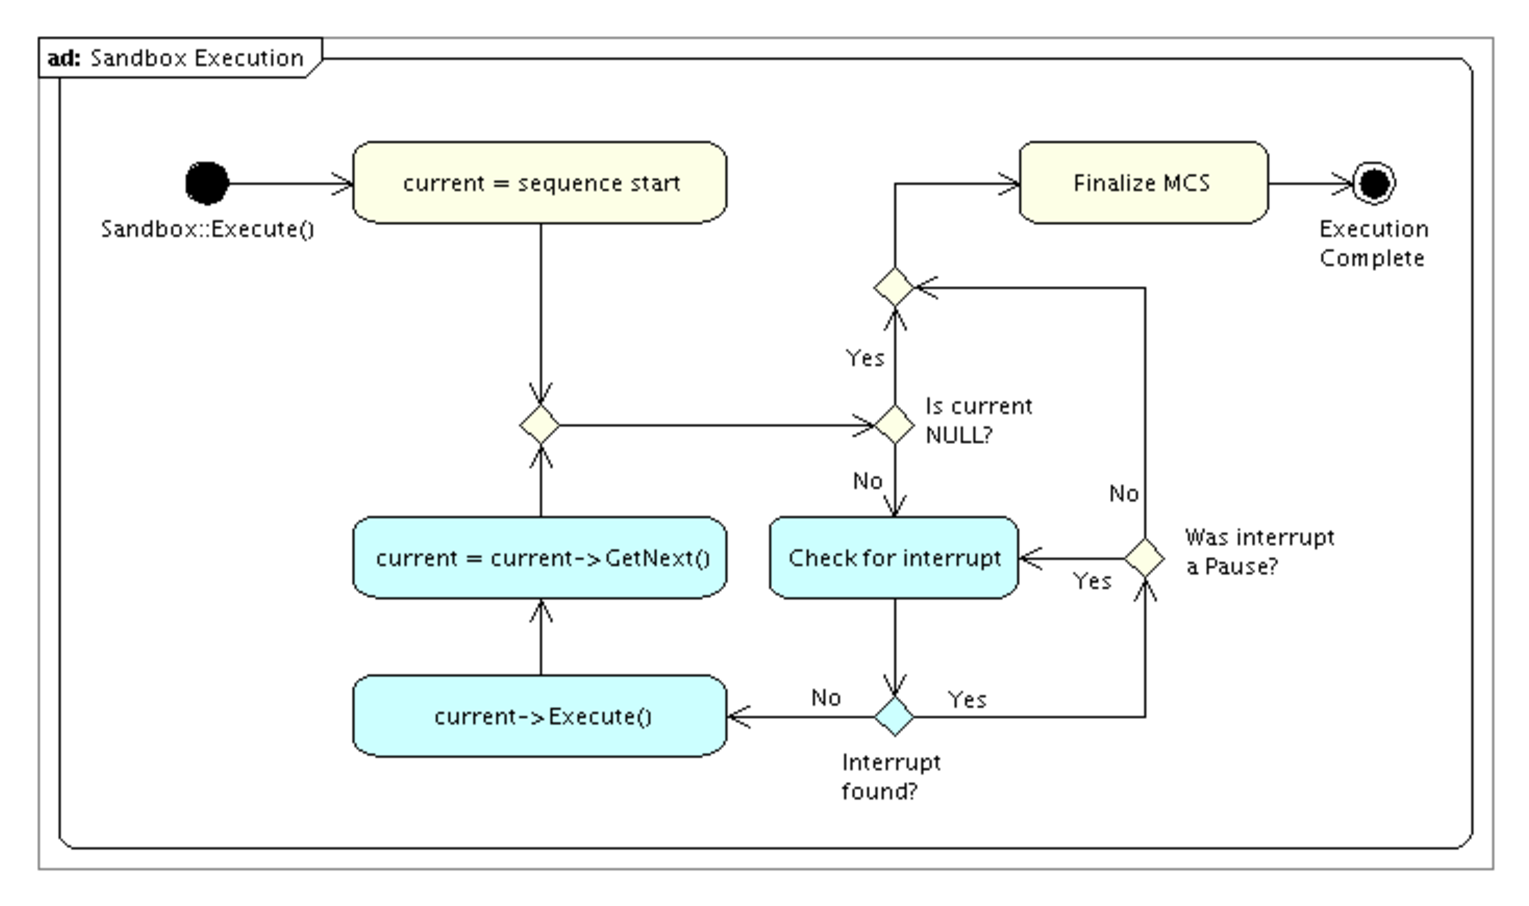
\includegraphics[scale=0.6]{Images/SandboxExecution.eps}
\caption{\label{fig:SandboxExecution}The Sandbox::Execute() Method}
\end{center}
\end{figure}

Figure~\ref{fig:SandboxExecution} shows the process GMAT follows when executing the Mission Control Sequence.  The Moderator launches the run through a call to the Sandbox's Execute() method.  That method sets a pointer to the first command in the Mission Control Sequence.  If that pointer is not
NULL, the Sandbox then places a callback to the Moderator to see if a user interrupt (typically a request to stop or pause the control sequence execution) has occurred.  If there is no interrupt, the command's Execute() method is called.  The command performs its processing, and returns control to the Sandbox.  The Sandbox then calls the command's GetNext() method, setting the command pointer to the next command that needs to be executed in the Mission Control Sequence.  If that pointer is not NULL, the Sandbox makes a callback to the Moderator to see if a user interrupt has occurred, and the process repeats. The run ends when the command pointer is set to NULL.  At that point, each command in the Mission Control Sequence is given the opportunity to finalize itself, and then control is returned to the Moderator, completing the run.

One subtlety in this process is the interplay between calls to a command's Execute() and GetNext() methods.  Some commands in GMAT -- particularly those that perform propagation and those that manage logical branching in the control sequence -- consume more computational time than desired before checking for user interrupts.  The implementation of the Execute() and GetNext() methods for these commands is designed to allow for interruption and reentry to the command so that interrupt checking can be performed while the command is executing.  At select times during execution of these commands, the process is paused and control is returned to the Sandbox.  The call to the GetNext() method in these cases returns a pointer to the executing command, rather than the next command in the Mission Control Sequence.  After the Sandbox performs the interrupt check, the command is called and execution resumes at the point where it was paused.

The commands that govern estimation -- specifically the RunEstimator, RunSimulator, and Estimate commands -- described in this document all exhibit this reentrant interrupt behavior.  The descriptions of those commands in the following sections include descriptions of this implementation in the descriptions of the execution process for the commands.

\begin{center}
\begin{tabular}{|p{1in}|p{1.5in}|p{3in}|}
\hline\mc{3}{|l|}{\cellcolor[rgb]{0.75,0.75,0.75}\textbf{GMAT Status After Calls to Execute() and
GetNext() are Complete}} \\
\hline\mc{3}{|p{5.5in}|}{GMAT has completed the run.  Each command in the Mission Control Sequence has been executed, with the possible exception of conditional branches that may have been skipped.  Command Summary data is available for each executed command.  The objects in the Sandbox have been used as dictated by the contents of the Mission Control Sequence.} \\
\hline\rowcolor[rgb]{0.9,0.9,0.9}\textbf{\textit{Object}} & \textbf{\textit{Status}} &
\textbf{\textit{Notes}} \\
\hline ODSat & Created and Exercised & Sandbox version of the ODSat object contains the results of
the estimation process \\
\hline MauiData & Created and Exercised &  \\
\hline BLS & Created and Exercised &  \\
\hline Maui & Created and Exercised &  \\
\hline ODProp & Created and Exercised &  \\
\hline RunEstimator & Executed Once & The command has been executed.  If the tracking data is
suitable, the estimator has run to completion and converged on a solution, which has been fed back into the resources in the Sandbox.\\
\hline
\end{tabular}
\end{center}
